\section{Đồ thị hàm số}
\dn{Đồ thị hàm số bậc 2}{
    \textbullet Trong chương trình học ta chỉ khảo sát hàm số bậc 2 có dạng $y=ax^2$ \xd 
    $(a \khac 0)$. \xd 
    \textbullet Hàm số bậc 2 nói chung đều có dạng một đường cong gọi là \textit{Parabol}. \xd 
    \textbullet Đường cong Parabol có hai loại: Úp lên ($a > 0$) hoặc úp xuống ($ a < 0$).
    }

  \begin{figure}[h]
		\subfloat[$(a > 0)$\label{hinh1a}]{\includegraphics[width=0.35\textwidth]{img/Do_thi_ham_so_bac_2a.pdf}}\hfill
		\subfloat[$(a < 0)$\label{hinh1b}]{\includegraphics[width=0.35\textwidth]{img/Do_thi_ham_so_bac_2b.pdf}}
		\caption{2 hình dạng Parabol}
		\label{hinh1.1}
\end{figure}

\subsection{Cách vẽ Parabol}
\ex{Cách vẽ Parabol}{
  Vẽ đồ thị hàm số: 
  \[
    \colorbox{themecolor!10!white}{$y = x^2$}
  \]
  Bước 1: Lập bảng giá trị \xd 
  	\begin{tabularx}{\textwidth}{CCCCCC}
    \arrayrulecolor{themecolor!40!white}
		\midrule
		$x$     & $-2$ & $-1$ & $0$ & $1$ & $2$ \\
    $y=x^2$ &  $4$ & $1$  & $0$ & $1$ & $4$ \\
    \midrule
	  \end{tabularx}
    \mn[-3.5\baselineskip]{
      Một số quy tắc khi lập bảng: \xd
      \textbullet Chọn các giá trị $x$ có tính đối xứng. \xd
      \textbullet Chọn các giá trị $x$ mà cho ra một kết quả $y$ dễ dàng vẽ.
       }

  Bước 2: Vẽ trục tọa độ $Oxy$
    \begin{center}
      \includegraphics[width=0.5\textwidth]{img/Truc_Oxy.pdf}
      \captionsetup{hypcap=false}
      \captionof{figure}{Trục $Oxy$}
      \label{hinh1.2}
    \end{center}
      \mn[-12\baselineskip]{
        Một số lưu ý khi vẽ trục: \xd 
        \textbullet Chỉ vẽ vừa đủ các giá trị, không vẽ quá nhiều giá trị không có trong bảng. \xd
        \textbullet Kích cỡ số vừa đủ, không vẽ quá to, để tốt hơn về mặt thị giác.
      }

  Bước 3: Vẽ các điểm có trong bảng lên trục $Oxy$ \xd
    \begin{center}
      \includegraphics[width=0.5\textwidth]{img/Truc_Oxy_co_diem.pdf}
      \captionsetup{hypcap=false}
      \captionof{figure}{Các điểm trên trục $Oxy$}
      \label{hinh1.3}
    \end{center}

  Bước 4: Sử dụng thước Parabol để vẽ
    \begin{center}
		  \includegraphics[width=0.3\textwidth]{img/Parabol_trai.pdf}\hfill
		  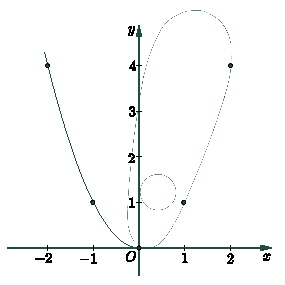
\includegraphics[width=0.3\textwidth]{img/Parabol_phai.pdf}\hfill
      \includegraphics[width=0.3\textwidth]{img/Parabol_full.pdf}
      \captionsetup{hypcap=false}
		  \captionof{figure}{Cách dùng thước Parabol để vẽ}
		  \label{hinh1.4}
    \end{center}
    \mn[-11.5\baselineskip]{
      Một số lưu ý khi sử dụng Parabol: \xd 
      \textbullet Parabol có hai đầu, ta lựa chọn 1 trong 2 đầu để vẽ. \xd 
      \textbullet Đỉnh của Parabol có xu hướng bị nhọn, điều này là bình thường do cấu tạo của thước, có thể sử dụng tay để đồ nhẹ lại đỉnh để tạo cảm giác cong. \xd 
      \textbullet Đỉnh của Parabol nếu quá nhọn sẽ bị trừ điểm.
      }    
}
